\chapter{Le immagini digitali}
\section{Definizione di immagine}
Useremo il Teorema del campionamento per applicarlo al concetto di immagine.
\begin{definition}
    Un’immagine è una rappresentazione grafica di valori numerici.
\end{definition}
In dettaglio un’immagine è una funzione bi-dimensionale $f(x,y)$, dove le
variabili (spaziali) $x$ e $y$ sono valori reali che definiscono la posizione
dei punti nell’immagine e $f(x,y)$ e in genere un valore reale che definisce
l’intensità dell’immagine nel punto $(x,y)$. \\Il punto che andiamo a definire
con le coordinare $x$, $y$ definisce il punto di grigio, al quale appartiene una
data intensità.\\

Tutti i colori al calcolatore possono essere scomposti
mediante combinazioni di 3 colori principali: \textbf{Rosso}, \textbf{Verde} e
\textbf{Blu} (\textbf{RGB}). Dove:

$$
    R = f_1, \ G = f_2, \ B = f_3
$$

\paragraph{Note:}
\begin{itemize}
    \item In natura i tutti i colori si ottengono a partire da \textbf{Rosso},
          \textbf{Giallo} e \textbf{Blu} (\textbf{RYB}), ma al computer possiamo ottenere
          un \textit{"giallo sintetico"} partendo dal Verde.
\end{itemize}

\section{Rappresentazione di un’immagine}
La funzione $f$ che rappresenta l’immagine può essere a valori in $\mathbb{R}$,
in $\mathbb{R}^2$ o in $\mathbb{R}^3$, a seconda del tipo di immagine. \TODO{Ricontrollare, $\mathbb{R}^2$ non ha senso}

\begin{itemize}
    \item \textbf{Immagine in scala di grigi:} $f:\mathbb{R}^2 \rightarrow \mathbb{R}$ (funzione
          scalare)
    \item \textbf{Immagine a colori:} $f:\mathbb{R}^2 \rightarrow \mathbb{R}^3$ (funzione
          vettoriale)
\end{itemize}

Ovvero:
\begin{center}
    $f(x,y) = [f_1(x,y), f_2(x,y), f_3(x,y)]$
\end{center}
dove le componenti $f_i$, $i = 1,2,3$ si dicono canali. \\\\Se vogliamo
rappresentare una scena in movimento, ottenendo cioè un' \textbf{immagine
    dinamica}, è necessario introdurre una terza variabile, quella
\textbf{temporale} ($t$), per cui si lavora con una funzione $f: \mathbb{R}^3 \rightarrow
    \mathbb{R}^3$.

$$
    f(x,y,t) = [f_1(x,y,t), f_2(x ,y,t), f_3(x,y,t)].
$$

Nelle immagini \textbf{Analogiche} conosco l'intensità di ogni livello di grigio
in ogni punto. Le immagini mostrate al calcolatore invece vanno
\textbf{DISCRETIZZATE!}!


\section{Discretizzazione}
Se si vuole utilizzare un calcolatore elettronico per lo studio di un segnale, è
necessario \textbf{discretizzare} la funzione $s(t)$ che rappresenta il segnale.
Infatti un calcolatore elettronico è in grado di trattare solo segnali discreti,
cioè successioni di campioni i cui valori sono rappresentati con precisione
finita. \\Se si lavora con un segnale continuo $s(t)$, per implementarne lo
studio al calcolatore è necessario passare ad un opportuno segnale discreto.

\begin{center}
    Ciò avviene utilizzando il procedimento di \textbf{campionamento}, che
    consiste nel discretizzare la variabile temporale $t$.
\end{center}

Inoltre, è anche necessario discretizzare i valori che la funzione $s(t)$ assume
(\textbf{quantizzazione}).\\

Nel caso delle immagini applicare i processi di \textbf{campionamento} e
\textbf{quantizzazione} significa passare da un'immagine \textbf{analogica} ad
un'immagine \textbf{digitale}.

\section{Campionamento di un segnale}
Il campionamento di un segnale può essere fatto in 2 diversi modi:
\begin{enumerate}
    \item \textbf{Nel tempo:} Il campionamento di un segnale si ottiene
          prelevando i valori che il segnale assume soltanto in istanti
          temporali fissati, in genere individuati tramite una funzione
          periodica \textbf{(funzione campionante)}. La successione dei valori
          campionati di s fornisce una rappresentazione \textbf{discreta} (nel
          tempo) di $s(t)$.
    \item \textbf{Nello spazio:} Un’immagine può essere vista come una funzione
          $f(x,y,t)$ dello spazio e del tempo e dunque è necessario
          discretizzare anche le variabili spaziali. Si ottiene in questo modo
          una matrice a tre dimensioni, delle quali due sono spaziali ed una è
          temporale.
\end{enumerate}
\section{Funzione Campionante}
In genere, si assume che il campionamento sia \textbf{uniforme}, sia dal punto
di vista spaziale che temporale, ovvero che la funzione campionante sia
periodica di periodo costante. \\\\Fissiamo gli intervalli di campionamento
$\Delta x$ , $\Delta y$, $\Delta t$ appropriati (dal Teorema Sampling e dalla
teoria di Nyquist), ovvero la distanza tra due campioni successivi lungo le
coordinate $x$, $y$ e $t$.\\Indichiamo con $N$, $M$, $T$ le dimensioni della
matrice dei valori campionati dell’immagine. Infine possiamo dare le seguenti

\begin{definition}
    La \textbf{funzione campionante} è
    $$
        s_c(x,y,t) = \sum_{j=1}^{M} \sum_{k=1}^{N}\sum_{h=1}^{T} \delta (x-j, y - k
        \Delta y, t - h  \Delta t )
    $$
\end{definition}

\begin{definition}
    L'\textbf{immagine campionata} è
    \begin{equation}
        \begin{aligned}
            s_c(x,y,t) & = f(x,y,t)s_c(x,y,t) =                                                                                \\
                       & = f(x,y,t) \sum_{j=1}^{M} \sum_{k=1}^{N}\sum_{h=1}^{T} \delta (x-j, y - k \Delta y, t - h  \Delta t )
        \end{aligned}
    \end{equation}
\end{definition}

Lo scopo della funzione campionante $s_c(x , y, t)$ è di prelevare i valori
campionati dal segnale continuo di partenza e pertanto ha un caratteristico
andamento \textbf{pulsante}.
\begin{itemize}
    \item Il segnale \textbf{non va mai letto}
          
          quando $x$ cade nel nodo della funzione in quanto non si sarebbe in
          grado di leggerlo.
    \item Il segnale \textbf{va letto}
          soltanto in $\frac{j}{w}$ ovvero la funzione campionante parallela ai
          campioni.
          \TODO[]{Ricontrollare questi 2 punti.}
\end{itemize}

%TODO: Inserire foto
\missingfigure{Inserire foto}

\section{Quantizzazione}
Per ottenere una completa discretizzazione di un’immagine è necessario
discretizzare, oltre al dominio, anche l’insieme immagine (insieme dei valori).
\begin{definition}
    Si definisce \textbf{quantizzazione} il procedimento di discretizzazione dei
    valori della funzione che rappresenta un’immagine, cioè il passaggio da
    valori continui a valori discreti.
\end{definition}
Per le immagini a toni di grigio si parla di \textbf{grey level quantization},
mentre per le immagini a colori si parla di \textbf{color depth}, in riferimento
al numero di bit utilizzati per ciascun canale di colore (8, 16, 24, 32 bit).
\begin{itemize}
    \item \textbf{Esempio 1:} \TODO[]{Si potrebbe aggiungere qualche altra informazione}
          Le immagini che siamo abituati a vedere tutti i giorni sui nostri cellulari
          sono immagini a colori a 8bit.
    \item \textbf{Esempio 2:} Nelle immagini mediche, di solito in formato
          \textbf{DICOM}, le immagini vengono rappresentate a 16bit ma gli
          ultimi 4 bit dell'immagine sono riservati ad informazioni personali
          che servono ad identificare il paziente che ha sostenuto l'esame.
\end{itemize}
\section{Immagine Digitale}
Tramite il campionamento e la quantizzazione è possibile definire un’immagine
digitale come segue:
\begin{definition}
    Una immagine digitale è una rappresentazione di matrici di elementi
    immagine, detti anche pixel (pixel = picture elements). Dove
    
    \begin{itemize}
        \item Il \textbf{pixel} costituisce la componente elementare della matrice,
              dove gli indici di riga e colonna indicano i valori delle due
              variabili spaziali, cioè la posizione di un punto nell’immagine.
        \item Ogni elemento della matrice contiene i valori che rappresentano
              l’intensità dei corrispondenti punti nell’immagine, anche detta
              \textbf{luminanza}.
    \end{itemize}
\end{definition}

\section{Teorema del Campionamento nelle Immagini}
L'Immagine campionata è rappresentata tramite la seguente formula:

$$
    s_c(x,y) = f(x,y)s_c(x,y)=f(x,y)\sum_{j=-\infty}^{+\infty}
    \sum_{k=-\infty}^{+\infty} \delta (x-j \Delta x, y-k \Delta y)
$$

dove $s_c(x,y)$ è \textbf{la funzione campionante}. \\\\Si può provare che c’è
una relazione tra $\hat{f}_c$ e $\hat{f}$. Per questo è importante assumere che
lo spettro del segnale $f$ sia \textbf{a banda limitata}, cioè:

$$
    \hat{f}(\omega_x, \omega_y)=0 \text{ per } |\omega_x| > \bar{\omega}_x \text{ e } |\omega_y| > \bar{\omega}_y
$$
dove $\bar{\omega}_x$ e $\bar{\omega}_y$ definiscono la banda rettangolare dell’immagine.
\\Così lo spettro dell’immagine campionata consiste nello spettro dell’immagine
continua infinitamente ripetuta nel piano delle frequenze, in una griglia di
risoluzione ($\frac{2\pi}{\Delta x}, \frac{2 \pi}{\Delta y}$), dove:

$$
    (\frac{2\pi}{\Delta x}, \frac{2 \pi}{\Delta y}) = (w_{xe}, w_{ye})
$$

sono le \textbf{frequenze Sampling}. \\\\Per ricostruire esattamente un segnale
campionato, la frequenza del campionamento non deve essere inferiore ad una
\textbf{frequenza minima (ovvero frequenza sampling)}, che corrisponde ad un
valore \TODO[]{Ricontrollare, prima viene detto 'valore massimo' e poi 'valore minimo'.}massimo per ciascuno degli intervalli $\Delta x$ , $\Delta y$. Tale
valore minimo deve essere almeno pari al doppio della banda massima di $f$ ,
cioè:

$$
    \omega_{xe} \geq 2 \bar{\omega}_x \text{ e } \omega_{ye} \geq 2 \bar{\omega}_y
$$

Se nella \TODO[]{Mo la (1) che è ?}(1) vale l’uguaglianza, allora si dice che l’immagine è
\textbf{campionata alla sua frequenza di Nyquist.}
\\\\Se $\Delta x$ e $\Delta y$ sono più piccoli del richiesto criterio di
Nyquist, l’immagine risulta sovracampionata \textbf{(oversampling)}. Nel caso
contrario, l’immagine non può essere ricostruita esattamente: si parla di
sottocampionamento \textbf{(undersampling)} e si presenta un fenomeno di
distorsione detto \textbf{aliasing.}

\paragraph{Note:}
\begin{itemize}
    \item il valore minimo è un valore puramente teorico. \\Nella pratica, non
          potendo in generale determinare con precisione la banda massima del
          segnale, si utilizzano frequenze di campionamento più alte. \\Spesso
          si campiona con una frequenza pari a 4 volte quella misurata.
\end{itemize}

\begin{theorem}
    Sia $f(x,y)$ una immagine
    \begin{itemize}
        \item  a banda limitata e ad energia finita, soddisfa quindi
              $$
                  \hat{f}(\omega_x,\omega_y) = 0 \text{ per } | \omega_x | >
                  \bar{\omega}_x \text{ e } | \omega_y | > \bar{\omega}_y;
              $$
        \item con $f$ uniformemente campionata in una
              griglia rettangolare con intervalli spaziali $\Delta x$, $\Delta y$,
        \item che abbia l'ordine di campionamento più grande dell'ordine di
              Nyquist, cioè
              $$
                  \omega_{xe} \geq 2 \bar{\omega}_x, \ \omega_{ye} \geq 2 \bar{\omega}_y
              $$
    \end{itemize}
    
    allora
    la $f$ può essere ricostruita dai suoi valori campione $f(j \Delta x, k
        \Delta y)$. Inoltre, l’immagine ricostruita è data dalla seguente formula di
    interpolazione:
\end{theorem}
\begin{center}
    $f(x,y) = \sum_{j=-\infty}^{+\infty} \sum_{k=-\infty}^{+\infty} f(j \Delta
        x, k \Delta y) (\frac{\sin(xw_{xe}-j)\pi}{(xw_{xe}-j)\pi})
        (\frac{\sin(yw_{ye}-k)\pi}{(yw_{ye}-k)\pi})$
\end{center}
\section{L'aliasing}
Per ricostruire esattamente una immagine, è necessario limitare in banda
l’immagine che deve essere campionata, campionando all’ordine di campionamento
di Nyquist o più grande e interpolando appropriatamente i valori immagine.
\\\\Se c’è sovrapposizione di spettri, risultante dal sottocampionamento, vuol
dire che componenti spettrali spurie sono state introdotte nel processo di
ricostruzione. L’effetto che si ottiene è chiamato aliasing.

%TODO: Inserire foto appunti fatti a mano 
\missingfigure{Inserire foto appunti fatti a mano }

Quindi l'aliasing è la presenza di componenti spettrali (frequenze) indesiderate
nella ricostruzione dell’immagine, componenti che non erano presenti quando
l’immagine originale era stata campionata.

\begin{figure}[H]
    \centering
    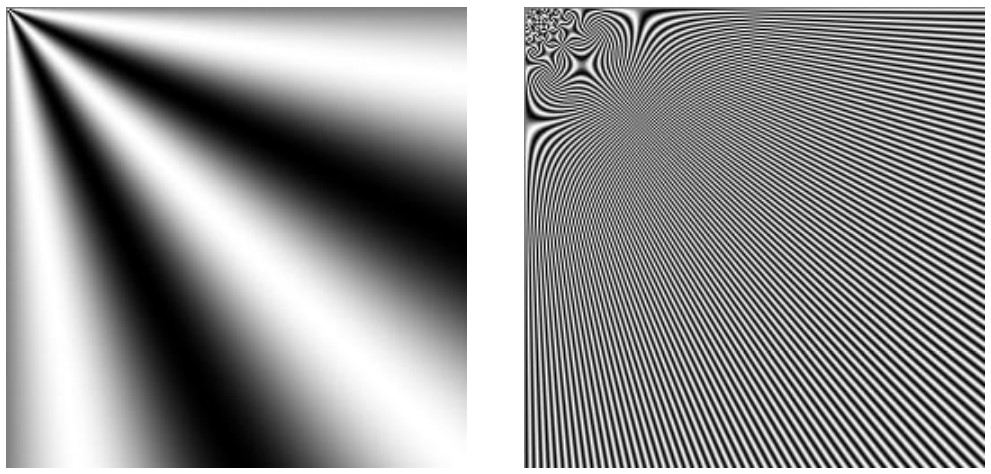
\includegraphics[width=10cm, keepaspectratio]{capitoli/immagini/imgs/aliasing_componenti_spettrali.jpg}
\end{figure}

L’aliasing deriva dal sottocampionamento e causa perdita di risoluzione
dell’immagine campionata (effetto scacchiera).

\begin{figure}[H]
    \centering
    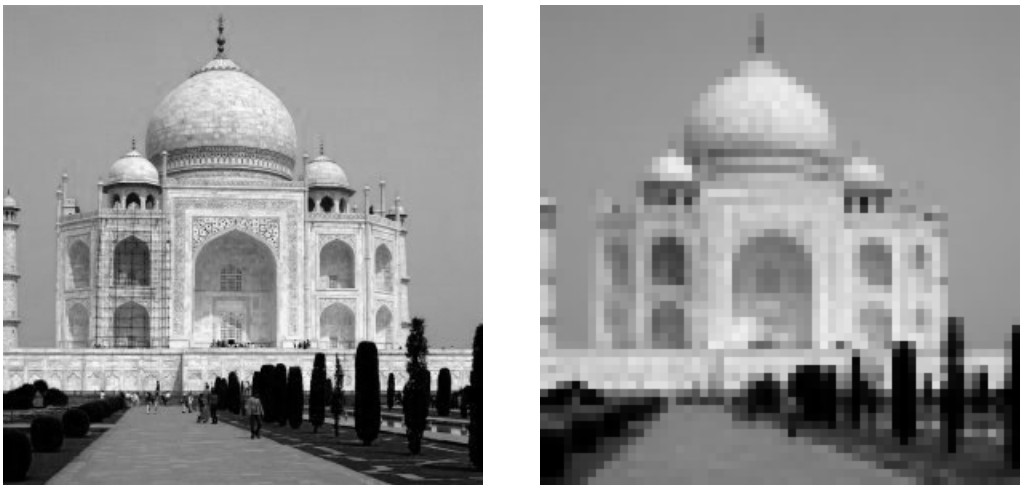
\includegraphics[width=10cm, keepaspectratio]{capitoli/immagini/imgs/aliasing_tajmahal.jpg}
\end{figure}

\paragraph{Note:} \TODO[]{Pricontrollare, potrebbe essere reso discorsivo.}
\begin{itemize}
    \item Per prevenire aliasing di queste componenti, è possibile filtrarle via
          (eliminarle) prima di campionare il segnale. Eliminare certe frequenze
          e lasciare passare le basse frequenze, è una operazione nota come
          \textbf{filtraggio passa-basso}.
    \item Ogni attenuazione relativa a questo processo di filtraggio rappresenta
          una perdita di risoluzione dell’immagine campionata.
    \item Come risultato, mentre da un lato c’è una perdita della risoluzione
          dell’immagine campionata, dall’altro c’è una attenuazione
          dell’aliasing error.
    \item \textbf{Effetto Moirè:} ovvero la distorsione visiva che si manifesta
          quando due griglie si sovrappongono
          \begin{figure}[H]
              \centering
              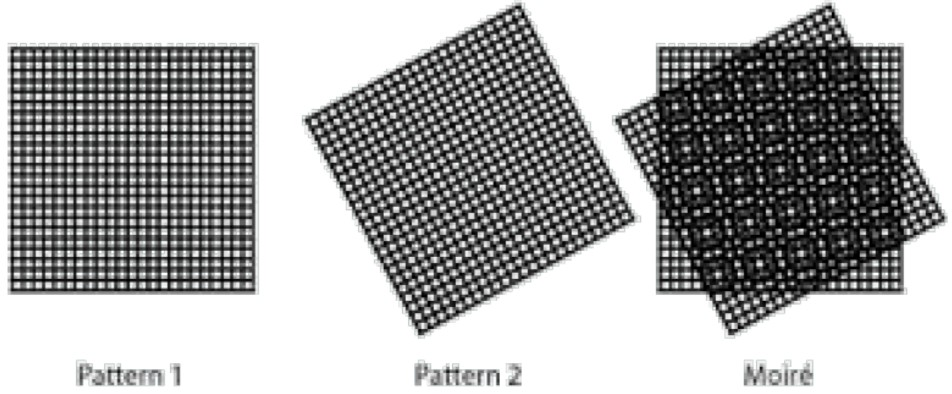
\includegraphics[width=8cm, keepaspectratio]{capitoli/immagini/imgs/effetto_moire.jpg}
          \end{figure}
\end{itemize}

\section{La risoluzione}
Il campionamento e la quantizzazione determinano la \textbf{risoluzione}
dell’immagine. \\\\La \textbf{risoluzione} di un segnale è un indice del grado
di qualità dell’immagine: misura il grado di oggetti distinguibili
nell’immagine. Esistono differenti definizione di risoluzione:

\begin{definition}
    La \textbf{Risoluzione Spaziale} indica la densità dei campioni, ovvero è data dal numero di campioni
    per unità di area.
\end{definition}

Spesso è espressa come numero di pixel
nell’unità di lunghezza e viene misurata in pixel per pollice (ppi).
\\Un’immagine ad alta risoluzione contiene più pixel di una delle
stesse dimensioni con una risoluzione inferiore, quindi è in grado di
riprodurre un maggior numero di dettagli. Un’elevata risoluzione
comporta tuttavia un aumento considerevole delle dimensioni (quantità
di dati) dell’immagine.

\paragraph{Esempio:}

Un’immagine di 1cm x 1cm con una risoluzione di 72 ppi
contiene 5184 pixel (72 x 72). La stessa immagine di 1 cm x
1 cm a 300 ppi conterrebbe 90.000 pixel.

\begin{definition}
    La \textbf{Risoluzione spettrale} indica la banda passante del sensore.
    
\end{definition}


\begin{definition}
    \textbf{Risoluzione radiometrica} indica il numero di livelli di quantizzazione.
    
\end{definition}


\begin{definition}
    \textbf{Risoluzione temporale} indica la frequenza di acquisizione dei frames di un’immagine in
    movimento.
\end{definition}



\section{Alterazioni della risoluzione}
Alterando i vari tipi di risoluzione, l’immagine presenterà di volta in volta un
diverso tipo di distorsione. \\ \textbf{Immagine originale:}

\begin{figure}[H]
    \centering
    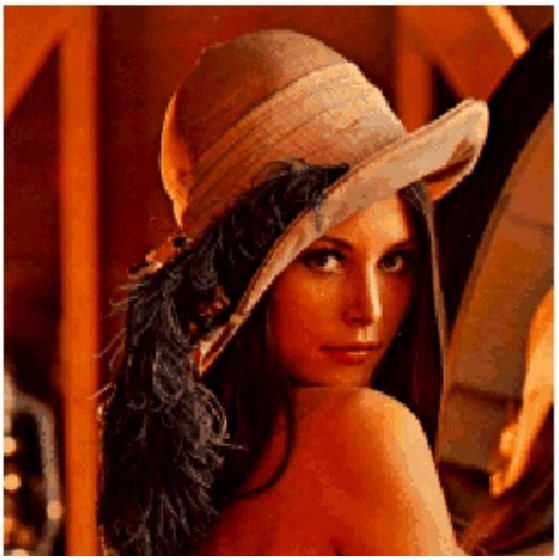
\includegraphics[width=4cm, keepaspectratio]{capitoli/immagini/imgs/alterazione_risoluzioni_esempio_base.jpg}
\end{figure}

\begin{trivlist}
    \item \textbf{Risoluzione spaziale:} diminuendo la risoluzione spaziale
    (nell’esempio di un quarto) si ottiene il tipico effetto ”quadrettato”,
    detto anche a scacchiera, dovuto all’aliasing.
    \begin{figure}[H]
        \centering
        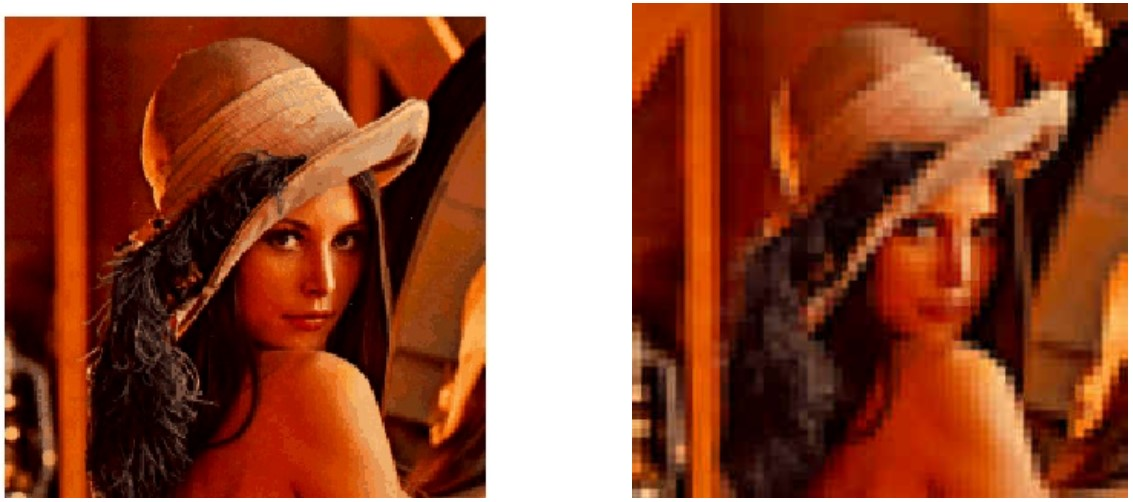
\includegraphics[width=10cm, keepaspectratio]{capitoli/immagini/imgs/esempio_risoluzione_spaziale.jpg}
    \end{figure}
    
    \item \textbf{Risoluzione spettrale:} Diminuendo la banda passante del
    sensore di acquisizione dell’immagine si ottiene un’immagine più ”sfocata”,
    in quanto i dettagli ad alta frequenza spaziale vanno persi.
    \begin{figure}[H]
        \centering
        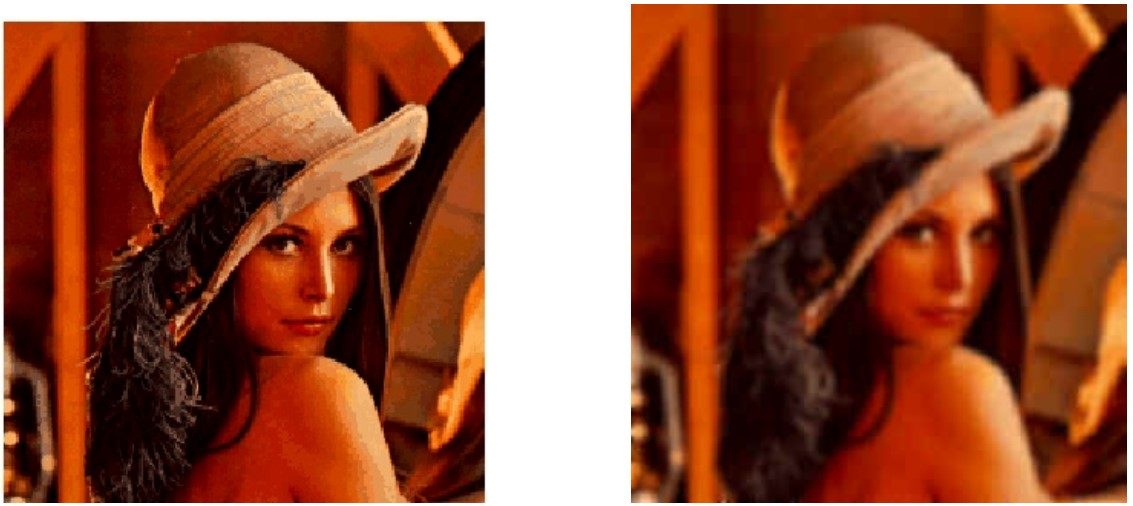
\includegraphics[width=10cm, keepaspectratio]{capitoli/immagini/imgs/esempio_risoluzione_spettrale.jpg}
    \end{figure}
    
    \item \textbf{Risoluzione radiometrica:} Diminuendo la profondità di colore,
    si distinguono in maniera più marcata i passaggi da un colore ad un altro;
    essi risultano pertanto sempre più accentuati e meno graduali, fino a
    produrre dei ”falsi contorni”
    \begin{figure}[H]
        \centering
        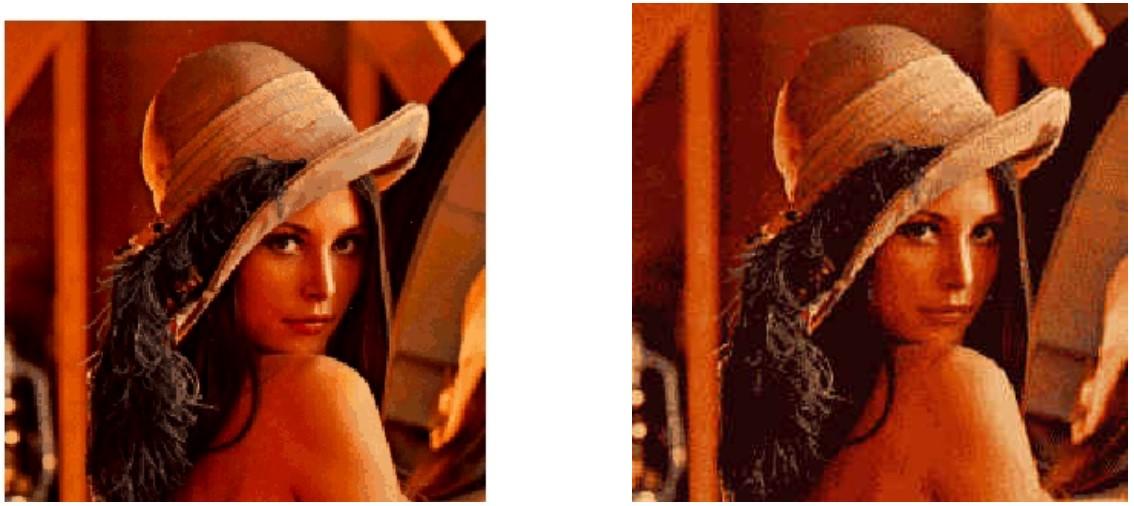
\includegraphics[width=10cm, keepaspectratio]{capitoli/immagini/imgs/esempio_risoluzione_radiometrica.jpg}
    \end{figure}
\end{trivlist}

\section{Immagini in bianco e nero e immagini a colori}

\subsection{Immagini in bianco e nero}

Un’\textbf{immagine in bianco e nero (b/w)} è caratterizzata da una
rappresentazione binaria, ovvero la funzione che la rappresenta in
ogni punto ($x$ , $y$) può assumere solo due valori: 0 e 1. In genere,
ad 1 si associa il bianco, mentre a 0 il nero.

\begin{figure}[H]
    \centering
    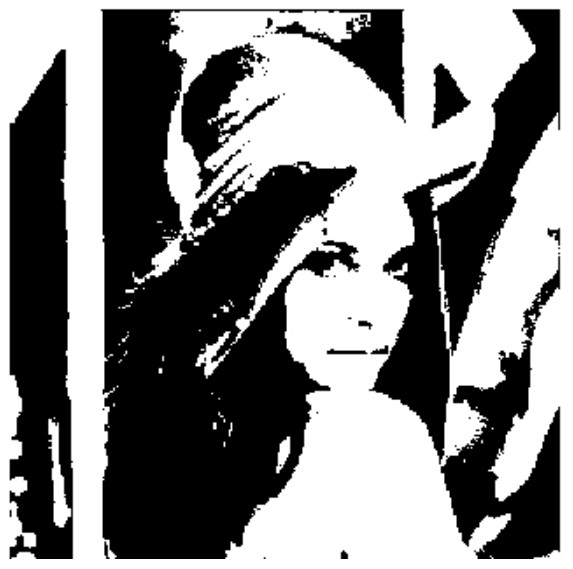
\includegraphics[width=4cm, keepaspectratio]{capitoli/immagini/imgs/immagine_binaria_bianco_nero.jpg}
\end{figure}

\subsection{Immagini a colori}

Per rappresentare un’\textbf{immagine a colori} è necessario ricorrere ad
una funzione vettoriale. Un colore infatti può essere sempre
decomposto come \textbf{somma dei tre colori fondamentali (rosso, verde,
    blu)}, ciascuno con un’opportuna intensità.
Un’immagine a colori, dunque, può essere rappresentata da una
funzione $f: \mathbb{R}^2 \rightarrow \mathbb{R}^3$ del tipo

$$
    f(x, y) = [R(x, y), G(x, y), B(x, y)]
$$

Questo tipo di rappresentazione viene detta \textbf{RGB (Red,Green,Blue)}.
\subsection{Lo spazio RGB}

Lo spazio RGB è uno spazio cartesiano, con tre assi ortogonali.
Il colore di ciascun pixel viene rappresentato da un vettore
$[R(x , y), G(x , y), B(x , y)]$ nello spazio RGB; ogni componente
indica la quantit`a di rosso, verde e blu, rispettivamente, necessari
ad ottenere quel colore.
In base alla rappresentazione RGB, un’immagine a colori viene
rappresentata da una terna di matrici, ognuna delle quali contiene i
valori relativi ad un canale di colore.\\
Ogni canale, preso a sè, non è altro che un’immagine a toni di
grigio.

\begin{figure}[H]
    \centering
    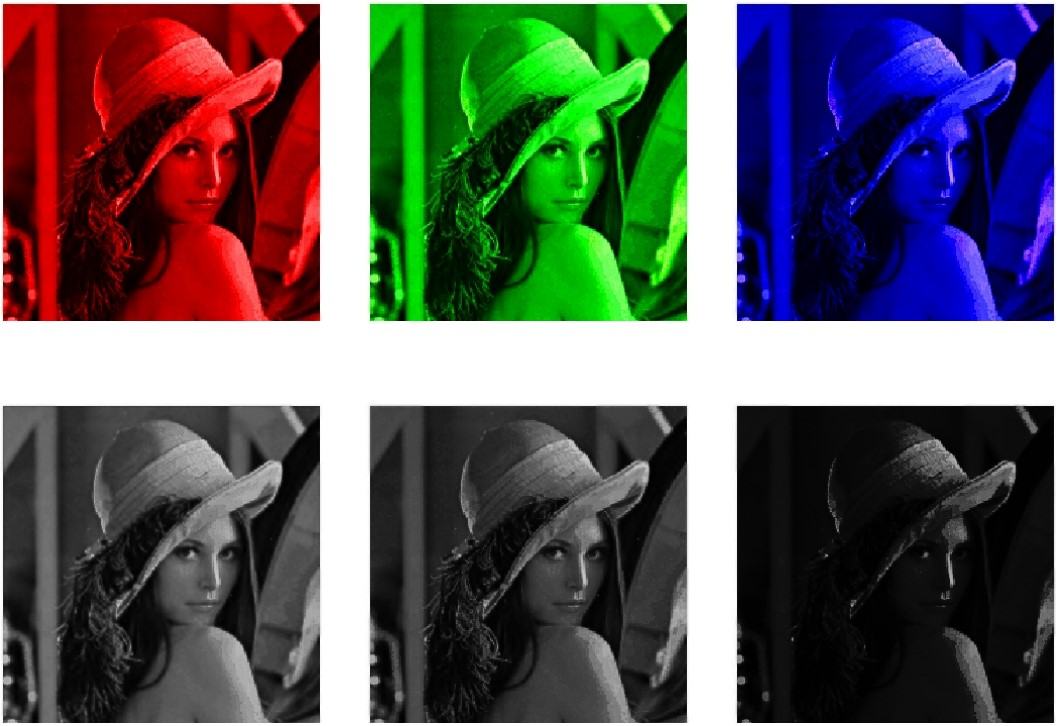
\includegraphics[width=12cm, keepaspectratio]{capitoli/immagini/imgs/canali_RGB_e_grigio.jpg}
\end{figure}

\subsection{Lo spazio HSV}

Oltre alla RGB esistono anche altri tipi di rappresentazioni (che
possono essere in genere derivate da essa).
Una di queste è la rappresentazione \textbf{HSV}. Lo spazio HSV ha un
sistema di coordinate cilindrico con due assi ortogonali ed un
angolo di rotazione intorno ad uno dei due assi.
L’altezza del cono rappresenta la \textbf{luminosità (Value)}, con valori da
0 (nero) a 1 (bianco). La \textbf{saturazione (Saturation)} indica l’intensità
e la purezza del colore, con valori da 0 (sull’asse del cono) a 1
(sulla superficie del cono). La terza coordinata rappresenta la
\textbf{tonalità di colore (Hue)} e viene misurata da un angolo intorno
all’asse verticale (rosso a 0 gradi, verde a 120 e blu a 240).

\begin{figure}[H]
    \centering
    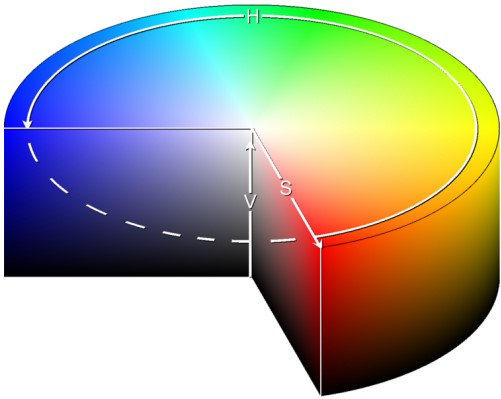
\includegraphics[width=5cm, keepaspectratio]{capitoli/immagini/imgs/cilindro_hsv.jpg}
\end{figure}

\section{Immagini a toni di grigio}

Un’immagine a toni di grigio è rappresentata da una matrice le cui
entrate sono i valori che la funzione $f$ assume in ogni punto.

\begin{figure}[H]
    \centering
    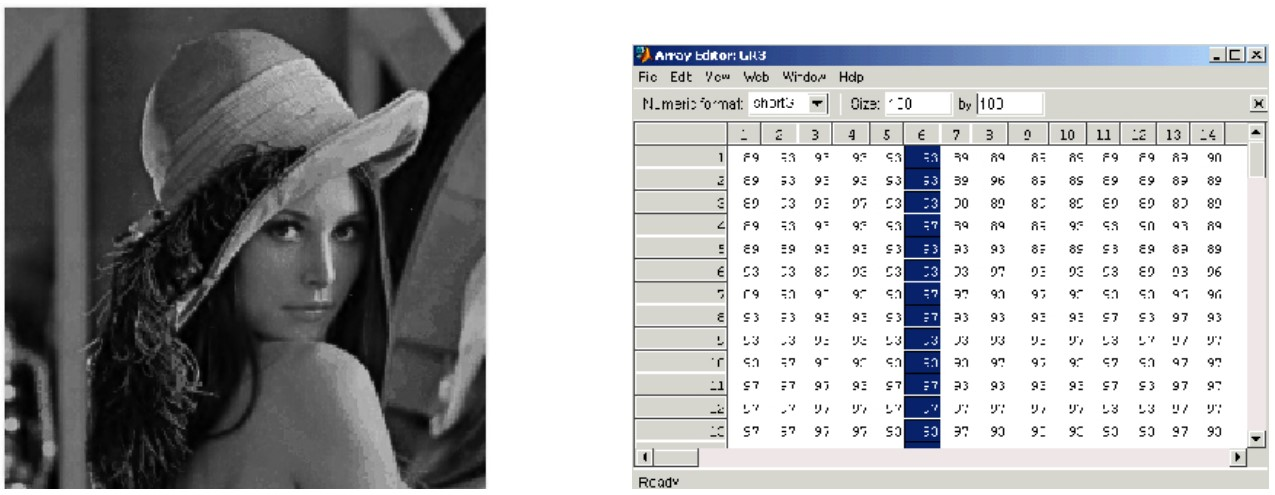
\includegraphics[width=12cm, keepaspectratio]{capitoli/immagini/imgs/rappresentazione_immagine_toni_grigio.jpg}
\end{figure}

In genere, si assume che i \textbf{livelli di grigio} siano discreti ed
equispaziati in un intervallo di valori normalmente \textbf{tra 0 e 255}:
esistono allora un massimo di 256 livelli di grigio.
\\
La funzione $f (x , y)$ può essere rappresentata come una superficie
nello spazio.

\begin{figure}[H]
    \centering
    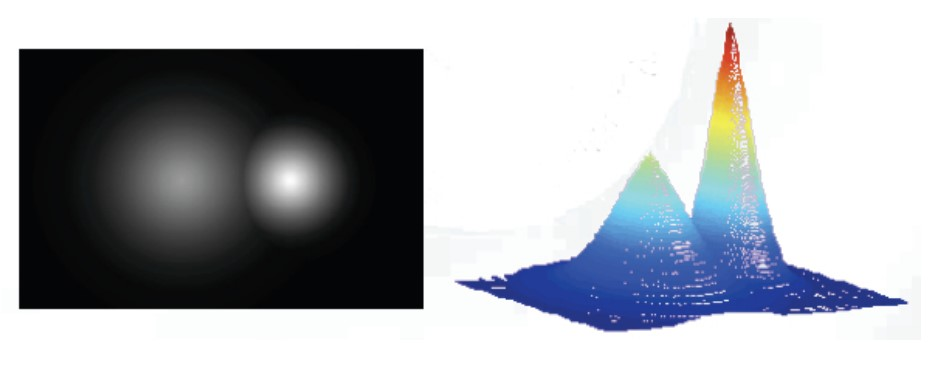
\includegraphics[width=10cm, keepaspectratio]{capitoli/immagini/imgs/funzione_toni_grigio.jpg}
\end{figure}

\subsection{Zoom e Shrink}

\textbf{DA IMPLEMENTARE QUANDO IL PROF LE SPIEGA}

\subsection{Elaborazione delle immagini}
L’elaborazione delle immagini è una disciplina che prevede l’utilizzo
di algoritmi i quali operano sui pixel che compongono l’immagine
e, applicando trasformazioni numeriche, restituiscono un’immagine
modificata.\\
Le tecniche di elaborazione delle immagini hanno vari scopi, fra cui:

\begin{itemize}
    \item il miglioramento della qualità dell’immagine (\textbf{image enhancement})
    \item il ripristino della qualità dell’immagine (\textbf{image restoration})
    \item l’estrazione di informazioni sul contenuto dell’immagine (\textbf{image analysis})
\end{itemize}

\textbf{Note:}\\

\begin{itemize}
    \item L’\textbf{image analysis} è una parte fondamentale della computer vision e
          precede l’\textbf{image recognition}.\\
          Essa può richiedere elaborazioni differenti a seconda del tipo di
          informazione che si vuole estrarre: tra queste, le elaborazioni nel
          dominio spaziale, nel dominio delle frequenze, con riduzione dei
          dati tra ingresso e uscita (compressione), etc.
\end{itemize}

\textbf{Esempio:}\\

Un’elaborazione nel dominio spaziale, ad esempio, può essere
espressa come

$$
    g(x , y) = T(f (x , y))
$$

\begin{itemize}
    \item $f$ è l’immagine di ingresso
    \item $g$ è l’immagine di uscita
    \item $T$ è un operatore su f, definito in un intorno di $(x , y)$.
\end{itemize}

La natura dell’intorno definisce il tipo di elaborazione e si distingue,
in particolare, fra: \textbf{elaborazioni puntuali}, \textbf{locali} e \textbf{globali}.

\begin{definition}
    Le elaborazioni \textbf{puntuali} trasformano il valore di un pixel sulla base del 
    valore del pixel stesso.
\end{definition}

\begin{definition}
    Le elaborazioni \textbf{locali} lavorano sulla base dei valori assunti dai pixel in 
    un intorno di quello preso in esame.
\end{definition}

\begin{definition}
    Le elaborazioni \textbf{globali} trasformano il valore di un pixel sulla
    base dei valori assunti da tutti i pixel dell’immagine.
\end{definition}

\subsubsection{Elaborazioni Puntuali}

\begin{definition}
    Un’elaborazione puntuale si dice \textbf{omogenea} se il risultato
    dipende solo dal valore del pixel a cui è applicata.\\
    Se invece il risultato dipende anche dalla posizione del pixel,
    l’elaborazione puntuale è \textbf{non omogenea}.
\end{definition}

\textbf{Note:}\\

Elaborazioni puntuali sono anche dette \textbf{manipolazioni della scala dei
    grigi}\\
Un’elaborazione puntuale omogenea può essere rappresentata da
una trasformazione

$$
    s = T(r)
$$

\begin{itemize}
    \item $r$ è il livello di grigio dell’immagine di ingresso
    \item $s$ è il livello di grigio dell’immagine in uscita
\end{itemize}
In base al tipo di funzione T si ottiene un tipo diverso di
trasformazione: a \textbf{gradino (threshold)}, a \textbf{rampa}, 
\textbf{lineare} a \textbf{tratti}...

\begin{figure}[H]
    \centering
    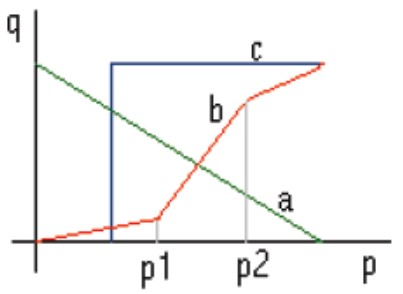
\includegraphics[width=5cm, keepaspectratio]{capitoli/immagini/imgs/elaborazioni_puntuali_immagine.jpg}
\end{figure}

\textbf{Esempio 1:}\\

Consideriamo una funzione T a gradino, ottenendo così una
\textbf{elaborazione threshold (soglia)}.\\
Tale elaborazione fa sì che i valori dei pixel che non superano la
soglia fissata vengano portato a 0, mentre i valori dei pixel che
superano la soglia siano posti pari a 1.\\
Si produce così un’immagine \textbf{binaria}.

\begin{figure}[H]
    \centering
    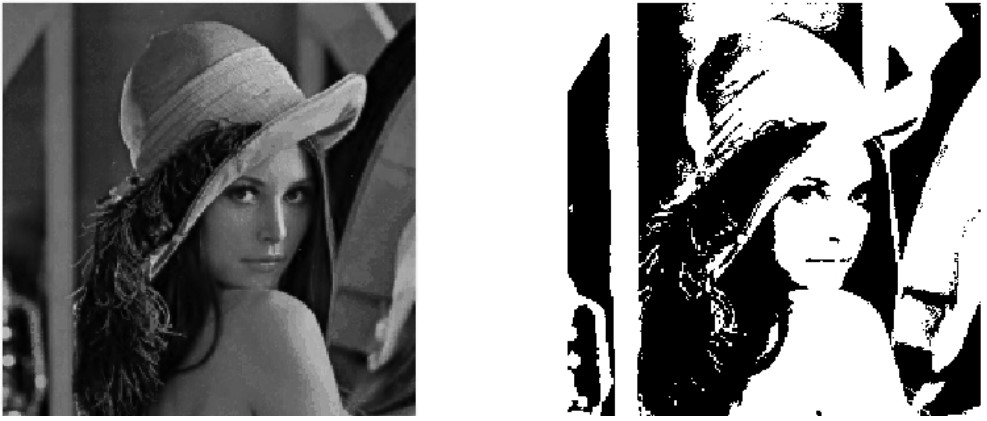
\includegraphics[width=10cm, keepaspectratio]{capitoli/immagini/imgs/foto_esempio_1.jpg}
\end{figure}

Questo è un tipico esempio di \textbf{binarizzazione}.
Si può ottenere una binarizzazione anche scegliendo una qualsiasi
altra \textbf{funzione di discriminazione}, invece di una soglia costante.

\textbf{Esempio 2:}\\

Consideriamo una $T$ del tipo:

\begin{figure}[H]
    \centering
    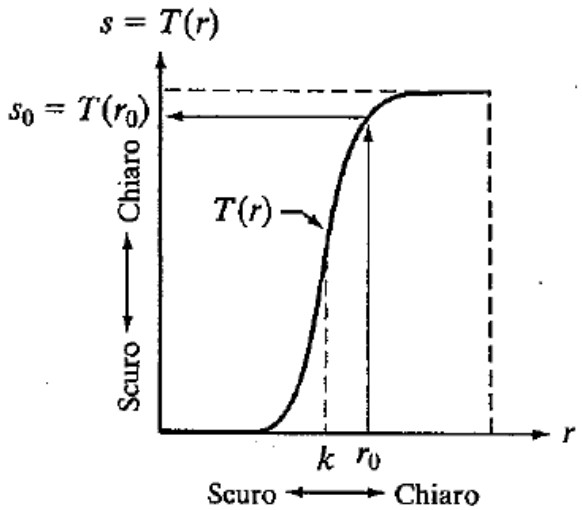
\includegraphics[width=6cm, keepaspectratio]{capitoli/immagini/imgs/trasformazione_esempio_2.jpg}
\end{figure}

Vengono scuriti i livelli di grigio al di sotto di $k$ e schiariti quelli al
di sopra di $k$. Si ottiene così uno \textbf{stiramento dell’immagine (image
    stretching)}. L’elaborazione threshold può essere riguardata come
caso limite di questo tipo di operazione.

\textbf{Esempio 3:}\\

Consideriamo una $T$ del tipo:

$$
    T(r) = L - 1 - r
$$

se il range dinamico dell’immagine è $[0, L - 1]$
la scala di grigi viene invertita, ottenendo così una negazione.

\begin{figure}[H]
    \centering
    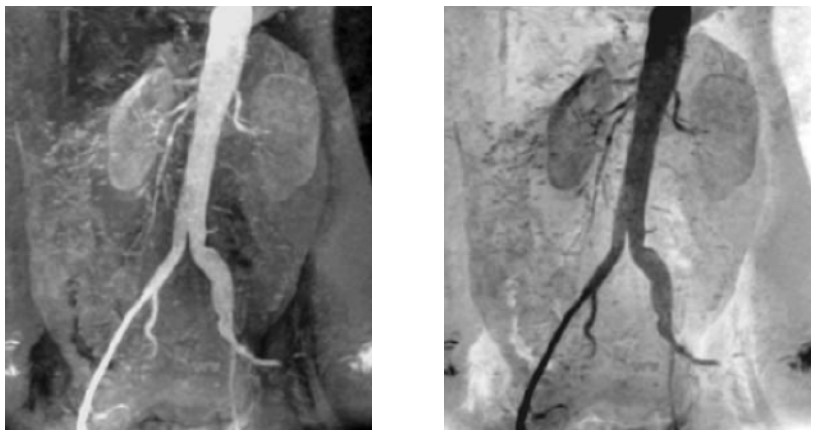
\includegraphics[width=8cm, keepaspectratio]{capitoli/immagini/imgs/angiografie_esempio_3.jpg}
\end{figure}

\textbf{Esempio 4:}\\

Consideriamo una $T$ del tipo:

$$
    T(r) = c \log(1 + r), c \in  \mathbb{R}, r \geq 0
$$

che prende il nome di \textbf{trasformazione logaritmica}: associa ad una
stretta gamma di valori a bassa intensità dell’immagine originale
una più ampia gamma nell’immagine in output.\\
Per livelli ad alta intensità, invece, si verifica il contrario.\\
Un tipico caso in cui è utile applicare questa trasformazione è per
rappresentare la trasformata di Fourier, che spesso presenta una
gamma molto ampia di intensità, difficilmente riproducibile senza
perdere un significativo livello di dettaglio

\begin{figure}[H]
    \centering
    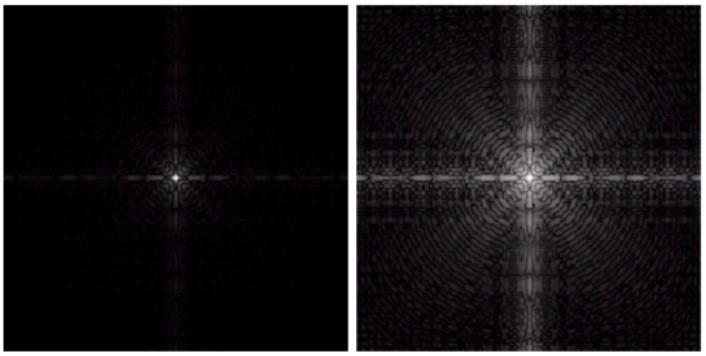
\includegraphics[width=10cm, keepaspectratio]{capitoli/immagini/imgs/trasformazione_logaritmica_esempio_4.jpg}
\end{figure}

\begin{itemize}
    \item Fig. sinistra: spettro di Fourier con valori in $[0, 1.5 \times 10^6]$.
    \item Fig. destra: risultato dell’applicazione della trasformazione logaritmica
          con $c = 1$ (valori in $[0, 6.2]$).
\end{itemize}

\textbf{Esempio 5:}\\

Consideriamo una $T$ del tipo:

$$
    T(r) = cr^\gamma, c, \gamma > 0,
$$

che prende il nome di \textbf{trasformazione di potenza (gamma)}
Se $\gamma < 1$ le curve potenza corrispondenti trasformano una stretta
gamma di valori scuri in una gamma più ampia di valori in output,
mentre se $\gamma > 1$, si verifica la trasformazione opposta.\\
La correzione tramite il fattore $\gamma$ è importante per la corretta
visualizzazione di immagini sullo schermo di un computer:
immagini non corrette nel modo giusto possono apparire sbiadite o,
al contrario, troppo scure.

\begin{figure}[H]
    \centering
    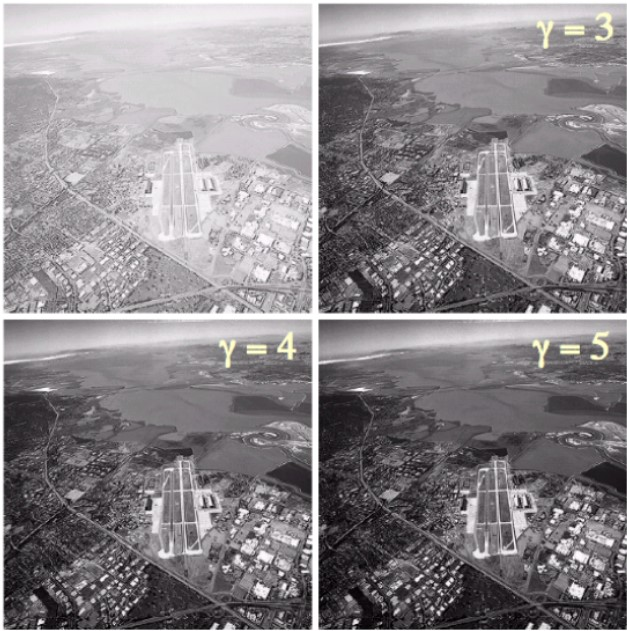
\includegraphics[width=6cm, keepaspectratio]{capitoli/immagini/imgs/foto_esempio_5.jpg}
\end{figure}

\textbf{Esempio 6:}\\

Considerando una $T$ \textbf{lineare a tratti} del tipo si ottiene uno 
stretching del contrasto

\begin{figure}[H]
    \centering
    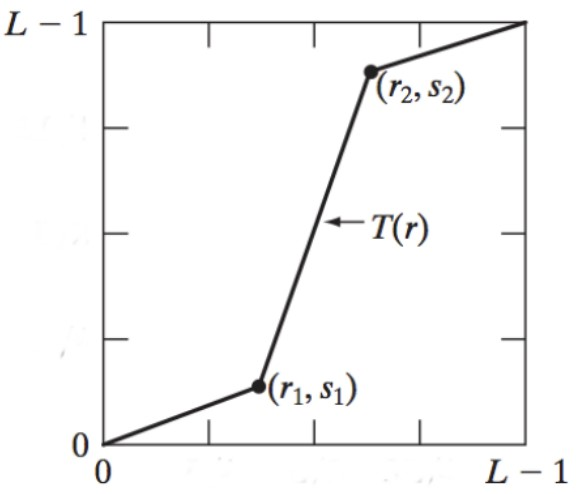
\includegraphics[width=5cm, keepaspectratio]{capitoli/immagini/imgs/lineare_a_tratti_esempio_6.jpg}
\end{figure}

In questo caso invece si ha uno stretching del contrasto differente perchè si
sceglie come $(r_1, s_1) = (r_{min}, 0)$ e $(r_2, s_2) = (r_{max} , L - 1)$

\begin{figure}[H]
    \centering
    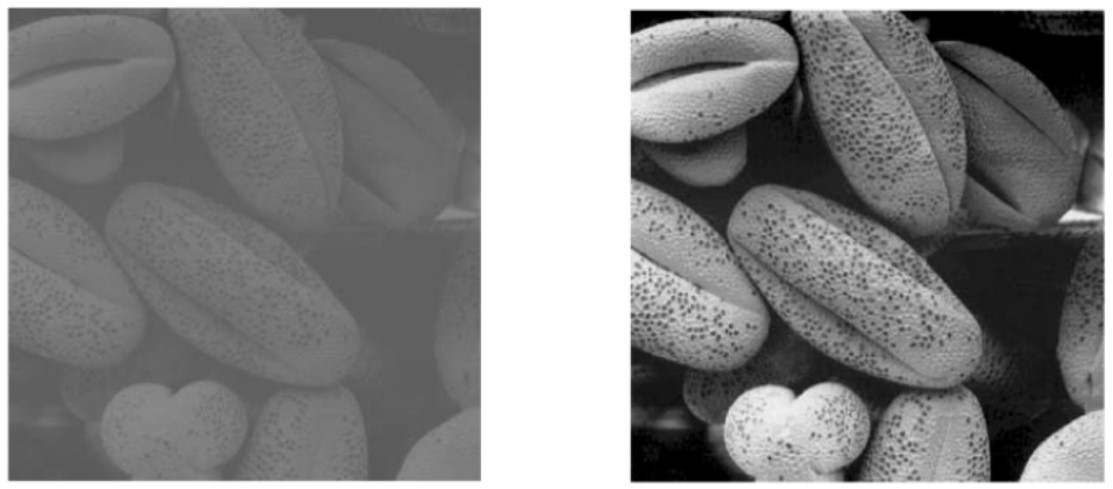
\includegraphics[width=10cm, keepaspectratio]{capitoli/immagini/imgs/globuli_rossi.jpg}
\end{figure}

\textbf{Note:}\\
In questo caso $r_{min}$ e $r_{max}$ stanno ad indicare il più basso e alto valore
nei livelli di grigio dell'immagine utilizzata.

\textbf{Esempio 7:}\\

\begin{figure}[H]
    \centering
    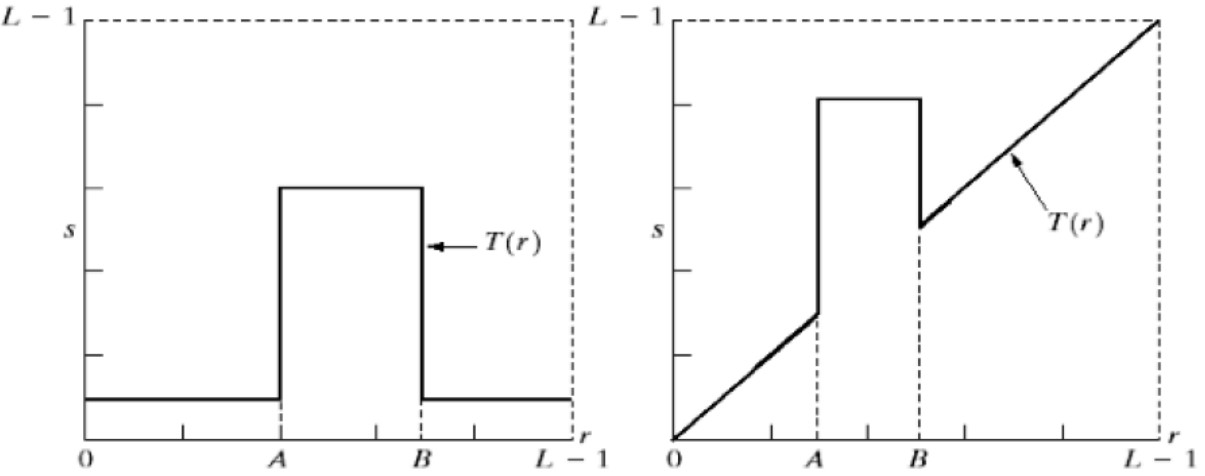
\includegraphics[width=\linewidth, keepaspectratio]{capitoli/immagini/imgs/trasformazioni_lineari_esempio_7.jpg}
\end{figure}

In questo caso prendiamo queste due diverse trasformazioni ed analizziamo il loro effetto sull'immagine.

\begin{itemize}
    \item La prima crea una binarizzazione ma in questo caso utilizza due differenti gradazioni di grigio e sono precisamente bianco e nero.
    \item La seconda mette in \textbf{risalto} una porzione della scala di grigi alzandogli il lvello e schiarendoli.
\end{itemize}

\begin{figure}[H]
    \centering
    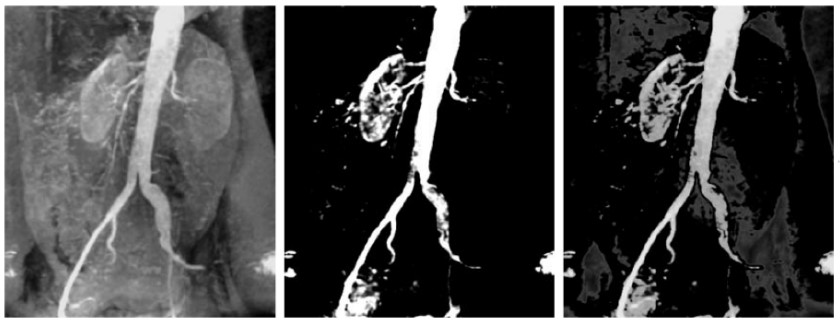
\includegraphics[width=\linewidth, keepaspectratio]{capitoli/immagini/imgs/angiografie_esempio_7.jpg}
\end{figure}

\begin{itemize}
    \item Nella prima immagine vediamo una normale Angiografia aortica.
    \item Nella seconda abbiamo il risultato della selezione di intensità del primo tipo (banda di
          interesse $[A, B]$ selezionata sulla parte alta della scala di grigi).
    \item Nella terza abbiamo il risultato della selezione di intensità del secondo tipo (banda
          $[A, B]$ sulle tonalità medio-grigie impostata sul nero, così da
          preservare le tonalità di grigio dei vasi e dei reni).
\end{itemize}